\documentclass[twoside]{book}

% Packages required by doxygen
\usepackage{fixltx2e}
\usepackage{calc}
\usepackage{doxygen}
\usepackage[export]{adjustbox} % also loads graphicx
\usepackage{graphicx}
\usepackage[utf8]{inputenc}
\usepackage{makeidx}
\usepackage{multicol}
\usepackage{multirow}
\PassOptionsToPackage{warn}{textcomp}
\usepackage{textcomp}
\usepackage[nointegrals]{wasysym}
\usepackage[table]{xcolor}

% Font selection
\usepackage[T1]{fontenc}
\usepackage[scaled=.90]{helvet}
\usepackage{courier}
\usepackage{amssymb}
\usepackage{sectsty}
\renewcommand{\familydefault}{\sfdefault}
\allsectionsfont{%
  \fontseries{bc}\selectfont%
  \color{darkgray}%
}
\renewcommand{\DoxyLabelFont}{%
  \fontseries{bc}\selectfont%
  \color{darkgray}%
}
\newcommand{\+}{\discretionary{\mbox{\scriptsize$\hookleftarrow$}}{}{}}

% Page & text layout
\usepackage{geometry}
\geometry{%
  a4paper,%
  top=2.5cm,%
  bottom=2.5cm,%
  left=2.5cm,%
  right=2.5cm%
}
\tolerance=750
\hfuzz=15pt
\hbadness=750
\setlength{\emergencystretch}{15pt}
\setlength{\parindent}{0cm}
\setlength{\parskip}{3ex plus 2ex minus 2ex}
\makeatletter
\renewcommand{\paragraph}{%
  \@startsection{paragraph}{4}{0ex}{-1.0ex}{1.0ex}{%
    \normalfont\normalsize\bfseries\SS@parafont%
  }%
}
\renewcommand{\subparagraph}{%
  \@startsection{subparagraph}{5}{0ex}{-1.0ex}{1.0ex}{%
    \normalfont\normalsize\bfseries\SS@subparafont%
  }%
}
\makeatother

% Headers & footers
\usepackage{fancyhdr}
\pagestyle{fancyplain}
\fancyhead[LE]{\fancyplain{}{\bfseries\thepage}}
\fancyhead[CE]{\fancyplain{}{}}
\fancyhead[RE]{\fancyplain{}{\bfseries\leftmark}}
\fancyhead[LO]{\fancyplain{}{\bfseries\rightmark}}
\fancyhead[CO]{\fancyplain{}{}}
\fancyhead[RO]{\fancyplain{}{\bfseries\thepage}}
\fancyfoot[LE]{\fancyplain{}{}}
\fancyfoot[CE]{\fancyplain{}{}}
\fancyfoot[RE]{\fancyplain{}{\bfseries\scriptsize Generated by Doxygen }}
\fancyfoot[LO]{\fancyplain{}{\bfseries\scriptsize Generated by Doxygen }}
\fancyfoot[CO]{\fancyplain{}{}}
\fancyfoot[RO]{\fancyplain{}{}}
\renewcommand{\footrulewidth}{0.4pt}
\renewcommand{\chaptermark}[1]{%
  \markboth{#1}{}%
}
\renewcommand{\sectionmark}[1]{%
  \markright{\thesection\ #1}%
}

% Indices & bibliography
\usepackage{natbib}
\usepackage[titles]{tocloft}
\setcounter{tocdepth}{3}
\setcounter{secnumdepth}{5}
\makeindex

% Hyperlinks (required, but should be loaded last)
\usepackage{ifpdf}
\ifpdf
  \usepackage[pdftex,pagebackref=true]{hyperref}
\else
  \usepackage[ps2pdf,pagebackref=true]{hyperref}
\fi
\hypersetup{%
  colorlinks=true,%
  linkcolor=blue,%
  citecolor=blue,%
  unicode%
}

% Custom commands
\newcommand{\clearemptydoublepage}{%
  \newpage{\pagestyle{empty}\cleardoublepage}%
}

\usepackage{caption}
\captionsetup{labelsep=space,justification=centering,font={bf},singlelinecheck=off,skip=4pt,position=top}

%===== C O N T E N T S =====

\begin{document}

% Titlepage & ToC
\hypersetup{pageanchor=false,
             bookmarksnumbered=true,
             pdfencoding=unicode
            }
\pagenumbering{alph}
\begin{titlepage}
\vspace*{7cm}
\begin{center}%
{\Large Assignment 2 -\/ Password Vault \\[1ex]\large 2 }\\
\vspace*{1cm}
{\large Generated by Doxygen 1.8.13}\\
\end{center}
\end{titlepage}
\clearemptydoublepage
\pagenumbering{roman}
\tableofcontents
\clearemptydoublepage
\pagenumbering{arabic}
\hypersetup{pageanchor=true}

%--- Begin generated contents ---
\chapter{Class Index}
\section{Class List}
Here are the classes, structs, unions and interfaces with brief descriptions\+:\begin{DoxyCompactList}
\item\contentsline{section}{\hyperlink{structBalancedBinTree}{Balanced\+Bin\+Tree} }{\pageref{structBalancedBinTree}}{}
\item\contentsline{section}{\hyperlink{structBalancedBinTreeNode}{Balanced\+Bin\+Tree\+Node} }{\pageref{structBalancedBinTreeNode}}{}
\end{DoxyCompactList}

\chapter{File Index}
\section{File List}
Here is a list of all documented files with brief descriptions\+:\begin{DoxyCompactList}
\item\contentsline{section}{include/\hyperlink{heap_8h}{heap.\+h} \\*File containing the function definitions of a heap }{\pageref{heap_8h}}{}
\item\contentsline{section}{include/{\bfseries heap\+A\+D\+T.\+h} }{\pageref{heapADT_8h}}{}
\item\contentsline{section}{include/\hyperlink{hospital_8h}{hospital.\+h} \\*File containing the extra function for Assignment 3 }{\pageref{hospital_8h}}{}
\item\contentsline{section}{include/\hyperlink{LinkedListAPI_8h}{Linked\+List\+A\+P\+I.\+h} \\*File containing the function definitions of a doubly linked list }{\pageref{LinkedListAPI_8h}}{}
\item\contentsline{section}{include/\hyperlink{QueueADT_8h}{Queue\+A\+D\+T.\+h} \\*File containing the function definitions of a queue }{\pageref{QueueADT_8h}}{}
\end{DoxyCompactList}

\chapter{Class Documentation}
\hypertarget{structHTable}{}\section{H\+Table Struct Reference}
\label{structHTable}\index{H\+Table@{H\+Table}}


{\ttfamily \#include $<$Hash\+Table\+A\+P\+I.\+h$>$}



Collaboration diagram for H\+Table\+:
\nopagebreak
\begin{figure}[H]
\begin{center}
\leavevmode
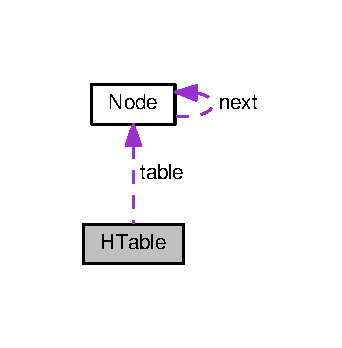
\includegraphics[width=164pt]{structHTable__coll__graph}
\end{center}
\end{figure}
\subsection*{Public Attributes}
\begin{DoxyCompactItemize}
\item 
\mbox{\Hypertarget{structHTable_a6ede6f5f1f743298425e0832cfd24a4a}\label{structHTable_a6ede6f5f1f743298425e0832cfd24a4a}} 
size\+\_\+t \hyperlink{structHTable_a6ede6f5f1f743298425e0832cfd24a4a}{size}
\begin{DoxyCompactList}\small\item\em number that represents the size of the hash table \end{DoxyCompactList}\item 
\mbox{\Hypertarget{structHTable_ad8f77b5519a173524eee87a5ebb380a0}\label{structHTable_ad8f77b5519a173524eee87a5ebb380a0}} 
\hyperlink{structNode}{Node} $\ast$$\ast$ \hyperlink{structHTable_ad8f77b5519a173524eee87a5ebb380a0}{table}
\begin{DoxyCompactList}\small\item\em array that contains all of the table nodes \end{DoxyCompactList}\item 
\mbox{\Hypertarget{structHTable_a05b3109f3bbfa3fd4b3e55c0bbd29b8a}\label{structHTable_a05b3109f3bbfa3fd4b3e55c0bbd29b8a}} 
void($\ast$ \hyperlink{structHTable_a05b3109f3bbfa3fd4b3e55c0bbd29b8a}{destroy\+Data} )(void $\ast$data)
\begin{DoxyCompactList}\small\item\em function pointer to a function to delete a single piece of data from the hash table \end{DoxyCompactList}\item 
\mbox{\Hypertarget{structHTable_a79abebe53db18bbf99f3938002b765e8}\label{structHTable_a79abebe53db18bbf99f3938002b765e8}} 
int($\ast$ \hyperlink{structHTable_a79abebe53db18bbf99f3938002b765e8}{hash\+Function} )(size\+\_\+t table\+Size, int key)
\begin{DoxyCompactList}\small\item\em function pointer to a function to hash the data \end{DoxyCompactList}\item 
\mbox{\Hypertarget{structHTable_a573abbe70757c842d491ff15d827c002}\label{structHTable_a573abbe70757c842d491ff15d827c002}} 
void($\ast$ \hyperlink{structHTable_a573abbe70757c842d491ff15d827c002}{print\+Data} )(void $\ast$to\+Be\+Printed)
\begin{DoxyCompactList}\small\item\em function pointer to a function that prints out a data element of the table \end{DoxyCompactList}\end{DoxyCompactItemize}


\subsection{Detailed Description}
Hash table structure 

The documentation for this struct was generated from the following file\+:\begin{DoxyCompactItemize}
\item 
include/\hyperlink{HashTableAPI_8h}{Hash\+Table\+A\+P\+I.\+h}\end{DoxyCompactItemize}

\hypertarget{structNode}{}\section{Node Struct Reference}
\label{structNode}\index{Node@{Node}}


{\ttfamily \#include $<$heap\+A\+D\+T.\+h$>$}



Collaboration diagram for Node\+:\nopagebreak
\begin{figure}[H]
\begin{center}
\leavevmode
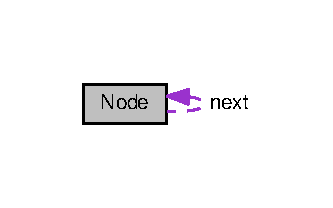
\includegraphics[width=166pt]{structNode__coll__graph}
\end{center}
\end{figure}
\subsection*{Public Attributes}
\begin{DoxyCompactItemize}
\item 
\mbox{\Hypertarget{structNode_a38b733496e3eff5e0b4fcb11cd9b866a}\label{structNode_a38b733496e3eff5e0b4fcb11cd9b866a}} 
void $\ast$ \hyperlink{structNode_a38b733496e3eff5e0b4fcb11cd9b866a}{data}
\begin{DoxyCompactList}\small\item\em contains void type data \end{DoxyCompactList}\item 
\mbox{\Hypertarget{structNode_ad0976834843c7618677d22a10c495b36}\label{structNode_ad0976834843c7618677d22a10c495b36}} 
struct \hyperlink{structNode}{Node} $\ast$ \hyperlink{structNode_ad0976834843c7618677d22a10c495b36}{left}
\begin{DoxyCompactList}\small\item\em contains left child node \end{DoxyCompactList}\item 
\mbox{\Hypertarget{structNode_af99e7102380da88d7c079fa264230cf4}\label{structNode_af99e7102380da88d7c079fa264230cf4}} 
struct \hyperlink{structNode}{Node} $\ast$ \hyperlink{structNode_af99e7102380da88d7c079fa264230cf4}{right}
\begin{DoxyCompactList}\small\item\em contains right child node \end{DoxyCompactList}\item 
\mbox{\Hypertarget{structNode_a34f3ab9670c7b70dad8905359a243c92}\label{structNode_a34f3ab9670c7b70dad8905359a243c92}} 
struct \hyperlink{structNode}{Node} $\ast$ \hyperlink{structNode_a34f3ab9670c7b70dad8905359a243c92}{parent}
\begin{DoxyCompactList}\small\item\em contains parent node \end{DoxyCompactList}\end{DoxyCompactItemize}


\subsection{Detailed Description}
Heap\+Node structure 

The documentation for this struct was generated from the following file\+:\begin{DoxyCompactItemize}
\item 
include/heap\+A\+D\+T.\+h\end{DoxyCompactItemize}

\chapter{File Documentation}
\hypertarget{HashTableAPI_8h}{}\section{include/\+Hash\+Table\+A\+PI.h File Reference}
\label{HashTableAPI_8h}\index{include/\+Hash\+Table\+A\+P\+I.\+h@{include/\+Hash\+Table\+A\+P\+I.\+h}}


File containing the function definitions of a hash table.  


{\ttfamily \#include $<$stdio.\+h$>$}\newline
{\ttfamily \#include $<$stdlib.\+h$>$}\newline
Include dependency graph for Hash\+Table\+A\+P\+I.\+h\+:
\nopagebreak
\begin{figure}[H]
\begin{center}
\leavevmode
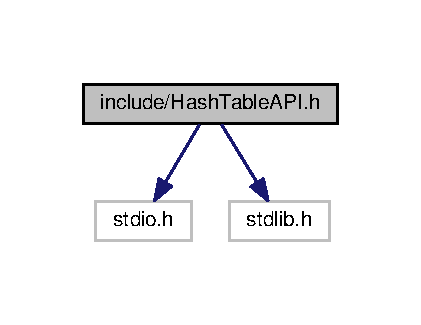
\includegraphics[width=202pt]{HashTableAPI_8h__incl}
\end{center}
\end{figure}
\subsection*{Classes}
\begin{DoxyCompactItemize}
\item 
struct \hyperlink{structNode}{Node}
\item 
struct \hyperlink{structHTable}{H\+Table}
\end{DoxyCompactItemize}
\subsection*{Typedefs}
\begin{DoxyCompactItemize}
\item 
typedef struct \hyperlink{structNode}{Node} \hyperlink{HashTableAPI_8h_a0466fc5f1bc9e6de776e48149b19c471}{Node}
\item 
typedef struct \hyperlink{structHTable}{H\+Table} \hyperlink{HashTableAPI_8h_a87a6d0849f5464aca79e337260a01316}{H\+Table}
\end{DoxyCompactItemize}
\subsection*{Functions}
\begin{DoxyCompactItemize}
\item 
\hyperlink{structHTable}{H\+Table} $\ast$ \hyperlink{HashTableAPI_8h_a7fdd867e4f213956eb6008d00f6e81d3}{create\+Table} (size\+\_\+t size, int($\ast$hash\+Function)(size\+\_\+t table\+Size, int key), void($\ast$destroy\+Data)(void $\ast$data), void($\ast$print\+Data)(void $\ast$to\+Be\+Printed))
\item 
\hyperlink{structNode}{Node} $\ast$ \hyperlink{HashTableAPI_8h_a9824e7141aa7a9bb4f08172ed6acd336}{create\+Node} (int key, void $\ast$data)
\item 
void \hyperlink{HashTableAPI_8h_a581f2ea930e7fb45ec8bb6f6dc959c01}{destroy\+Table} (\hyperlink{structHTable}{H\+Table} $\ast$hash\+Table)
\item 
void \hyperlink{HashTableAPI_8h_a3f4f20013b61c66b2642ce7681bf2667}{insert\+Data} (\hyperlink{structHTable}{H\+Table} $\ast$hash\+Table, int key, void $\ast$data)
\item 
void \hyperlink{HashTableAPI_8h_aad84519dd5dac14a07c42933296cacde}{remove\+Data} (\hyperlink{structHTable}{H\+Table} $\ast$hash\+Table, int key)
\item 
void $\ast$ \hyperlink{HashTableAPI_8h_a9b20212495eeff92430b5e570f085eee}{lookup\+Data} (\hyperlink{structHTable}{H\+Table} $\ast$hash\+Table, int key)
\end{DoxyCompactItemize}


\subsection{Detailed Description}
File containing the function definitions of a hash table. 

\begin{DoxyAuthor}{Author}
Michael Ellis 
\end{DoxyAuthor}
\begin{DoxyDate}{Date}
February 2017 
\end{DoxyDate}


\subsection{Typedef Documentation}
\mbox{\Hypertarget{HashTableAPI_8h_a87a6d0849f5464aca79e337260a01316}\label{HashTableAPI_8h_a87a6d0849f5464aca79e337260a01316}} 
\index{Hash\+Table\+A\+P\+I.\+h@{Hash\+Table\+A\+P\+I.\+h}!H\+Table@{H\+Table}}
\index{H\+Table@{H\+Table}!Hash\+Table\+A\+P\+I.\+h@{Hash\+Table\+A\+P\+I.\+h}}
\subsubsection{\texorpdfstring{H\+Table}{HTable}}
{\footnotesize\ttfamily typedef struct \hyperlink{structHTable}{H\+Table} \hyperlink{structHTable}{H\+Table}}

Hash table structure \mbox{\Hypertarget{HashTableAPI_8h_a0466fc5f1bc9e6de776e48149b19c471}\label{HashTableAPI_8h_a0466fc5f1bc9e6de776e48149b19c471}} 
\index{Hash\+Table\+A\+P\+I.\+h@{Hash\+Table\+A\+P\+I.\+h}!Node@{Node}}
\index{Node@{Node}!Hash\+Table\+A\+P\+I.\+h@{Hash\+Table\+A\+P\+I.\+h}}
\subsubsection{\texorpdfstring{Node}{Node}}
{\footnotesize\ttfamily typedef struct \hyperlink{structNode}{Node}  \hyperlink{structNode}{Node}}

\hyperlink{structNode}{Node} of the hash table. 

\subsection{Function Documentation}
\mbox{\Hypertarget{HashTableAPI_8h_a9824e7141aa7a9bb4f08172ed6acd336}\label{HashTableAPI_8h_a9824e7141aa7a9bb4f08172ed6acd336}} 
\index{Hash\+Table\+A\+P\+I.\+h@{Hash\+Table\+A\+P\+I.\+h}!create\+Node@{create\+Node}}
\index{create\+Node@{create\+Node}!Hash\+Table\+A\+P\+I.\+h@{Hash\+Table\+A\+P\+I.\+h}}
\subsubsection{\texorpdfstring{create\+Node()}{createNode()}}
{\footnotesize\ttfamily \hyperlink{structNode}{Node}$\ast$ create\+Node (\begin{DoxyParamCaption}\item[{int}]{key,  }\item[{void $\ast$}]{data }\end{DoxyParamCaption})}

Function for creating a node for the hash table. \begin{DoxyPrecond}{Precondition}
\hyperlink{structNode}{Node} must be cast to void pointer before being added. 
\end{DoxyPrecond}
\begin{DoxyPostcond}{Postcondition}
\hyperlink{structNode}{Node} is valid and able to be added to the hash table 
\end{DoxyPostcond}

\begin{DoxyParams}{Parameters}
{\em key} & integer that represents the data (eg 35-\/$>$\char`\"{}hello\char`\"{}) \\
\hline
{\em data} & is a generic pointer to any data type. \\
\hline
\end{DoxyParams}
\begin{DoxyReturn}{Returns}
returns a node for the hash table 
\end{DoxyReturn}
\mbox{\Hypertarget{HashTableAPI_8h_a7fdd867e4f213956eb6008d00f6e81d3}\label{HashTableAPI_8h_a7fdd867e4f213956eb6008d00f6e81d3}} 
\index{Hash\+Table\+A\+P\+I.\+h@{Hash\+Table\+A\+P\+I.\+h}!create\+Table@{create\+Table}}
\index{create\+Table@{create\+Table}!Hash\+Table\+A\+P\+I.\+h@{Hash\+Table\+A\+P\+I.\+h}}
\subsubsection{\texorpdfstring{create\+Table()}{createTable()}}
{\footnotesize\ttfamily \hyperlink{structHTable}{H\+Table}$\ast$ create\+Table (\begin{DoxyParamCaption}\item[{size\+\_\+t}]{size,  }\item[{int($\ast$)(size\+\_\+t table\+Size, int key)}]{hash\+Function,  }\item[{void($\ast$)(void $\ast$data)}]{destroy\+Data,  }\item[{void($\ast$)(void $\ast$to\+Be\+Printed)}]{print\+Data }\end{DoxyParamCaption})}

Function to point the hash table to the appropriate functions. Allocates memory to the struct and table based on the size given. \begin{DoxyReturn}{Returns}
pointer to the hash table 
\end{DoxyReturn}

\begin{DoxyParams}{Parameters}
{\em size} & size of the hash table \\
\hline
{\em hash\+Function} & function pointer to a function to hash the data \\
\hline
{\em destroy\+Data} & function pointer to a function to delete a single piece of data from the hash table \\
\hline
{\em print\+Node} & function pointer to a function that prints out a data element of the table \\
\hline
\end{DoxyParams}
\mbox{\Hypertarget{HashTableAPI_8h_a581f2ea930e7fb45ec8bb6f6dc959c01}\label{HashTableAPI_8h_a581f2ea930e7fb45ec8bb6f6dc959c01}} 
\index{Hash\+Table\+A\+P\+I.\+h@{Hash\+Table\+A\+P\+I.\+h}!destroy\+Table@{destroy\+Table}}
\index{destroy\+Table@{destroy\+Table}!Hash\+Table\+A\+P\+I.\+h@{Hash\+Table\+A\+P\+I.\+h}}
\subsubsection{\texorpdfstring{destroy\+Table()}{destroyTable()}}
{\footnotesize\ttfamily void destroy\+Table (\begin{DoxyParamCaption}\item[{\hyperlink{structHTable}{H\+Table} $\ast$}]{hash\+Table }\end{DoxyParamCaption})}

Deletes the entire hash table and frees memory of every element. \begin{DoxyPrecond}{Precondition}
Hash Table must exist. 
\end{DoxyPrecond}

\begin{DoxyParams}{Parameters}
{\em hash\+Table} & pointer to hash table containing elements of data \\
\hline
\end{DoxyParams}
\mbox{\Hypertarget{HashTableAPI_8h_a3f4f20013b61c66b2642ce7681bf2667}\label{HashTableAPI_8h_a3f4f20013b61c66b2642ce7681bf2667}} 
\index{Hash\+Table\+A\+P\+I.\+h@{Hash\+Table\+A\+P\+I.\+h}!insert\+Data@{insert\+Data}}
\index{insert\+Data@{insert\+Data}!Hash\+Table\+A\+P\+I.\+h@{Hash\+Table\+A\+P\+I.\+h}}
\subsubsection{\texorpdfstring{insert\+Data()}{insertData()}}
{\footnotesize\ttfamily void insert\+Data (\begin{DoxyParamCaption}\item[{\hyperlink{structHTable}{H\+Table} $\ast$}]{hash\+Table,  }\item[{int}]{key,  }\item[{void $\ast$}]{data }\end{DoxyParamCaption})}

Inserts a \hyperlink{structNode}{Node} in the hash table. \begin{DoxyPrecond}{Precondition}
hash\+Table type must exist and have data allocated to it 
\end{DoxyPrecond}

\begin{DoxyParams}{Parameters}
{\em hash\+Table} & pointer to the hash table \\
\hline
{\em key} & integer that represents the data (eg 35-\/$>$\char`\"{}hello\char`\"{}) \\
\hline
{\em data} & pointer to generic data that is to be inserted into the list \\
\hline
\end{DoxyParams}
\mbox{\Hypertarget{HashTableAPI_8h_a9b20212495eeff92430b5e570f085eee}\label{HashTableAPI_8h_a9b20212495eeff92430b5e570f085eee}} 
\index{Hash\+Table\+A\+P\+I.\+h@{Hash\+Table\+A\+P\+I.\+h}!lookup\+Data@{lookup\+Data}}
\index{lookup\+Data@{lookup\+Data}!Hash\+Table\+A\+P\+I.\+h@{Hash\+Table\+A\+P\+I.\+h}}
\subsubsection{\texorpdfstring{lookup\+Data()}{lookupData()}}
{\footnotesize\ttfamily void$\ast$ lookup\+Data (\begin{DoxyParamCaption}\item[{\hyperlink{structHTable}{H\+Table} $\ast$}]{hash\+Table,  }\item[{int}]{key }\end{DoxyParamCaption})}

Function to return the data from the key given. \begin{DoxyPrecond}{Precondition}
The hash table exists and has memory allocated to it 
\end{DoxyPrecond}

\begin{DoxyParams}{Parameters}
{\em hash\+Table} & pointer to the hash table containing data nodes \\
\hline
{\em key} & integer that represents a piece of data in the table (eg 35-\/$>$\char`\"{}hello\char`\"{}) \\
\hline
\end{DoxyParams}
\begin{DoxyReturn}{Returns}
returns a pointer to the data in the hash table. Returns N\+U\+LL if no match is found. 
\end{DoxyReturn}
\mbox{\Hypertarget{HashTableAPI_8h_aad84519dd5dac14a07c42933296cacde}\label{HashTableAPI_8h_aad84519dd5dac14a07c42933296cacde}} 
\index{Hash\+Table\+A\+P\+I.\+h@{Hash\+Table\+A\+P\+I.\+h}!remove\+Data@{remove\+Data}}
\index{remove\+Data@{remove\+Data}!Hash\+Table\+A\+P\+I.\+h@{Hash\+Table\+A\+P\+I.\+h}}
\subsubsection{\texorpdfstring{remove\+Data()}{removeData()}}
{\footnotesize\ttfamily void remove\+Data (\begin{DoxyParamCaption}\item[{\hyperlink{structHTable}{H\+Table} $\ast$}]{hash\+Table,  }\item[{int}]{key }\end{DoxyParamCaption})}

Function to remove a node from the hash table \begin{DoxyPrecond}{Precondition}
Hash table must exist and have memory allocated to it 
\end{DoxyPrecond}
\begin{DoxyPostcond}{Postcondition}
\hyperlink{structNode}{Node} at key will be removed from the hash table if it exists. 
\end{DoxyPostcond}

\begin{DoxyParams}{Parameters}
{\em hash\+Table} & pointer to the hash table struct \\
\hline
{\em key} & integer that represents a piece of data in the table (eg 35-\/$>$\char`\"{}hello\char`\"{}) \\
\hline
\end{DoxyParams}

\hypertarget{PasswordVault_8h}{}\section{include/\+Password\+Vault.h File Reference}
\label{PasswordVault_8h}\index{include/\+Password\+Vault.\+h@{include/\+Password\+Vault.\+h}}


File containing the function definitions for a password vault.  


{\ttfamily \#include \char`\"{}Hash\+Table\+A\+P\+I.\+h\char`\"{}}\newline
{\ttfamily \#include $<$stdio.\+h$>$}\newline
{\ttfamily \#include $<$stdlib.\+h$>$}\newline
Include dependency graph for Password\+Vault.\+h\+:
\nopagebreak
\begin{figure}[H]
\begin{center}
\leavevmode
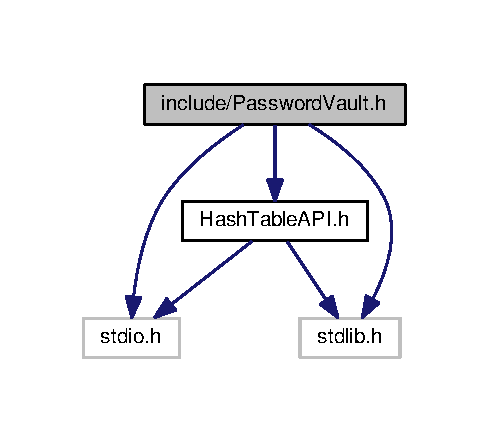
\includegraphics[width=235pt]{PasswordVault_8h__incl}
\end{center}
\end{figure}
\subsection*{Functions}
\begin{DoxyCompactItemize}
\item 
int \hyperlink{PasswordVault_8h_a21b3b10a074766df9adb5f02b4ea2f02}{hash\+Function} (size\+\_\+t table\+Size, char $\ast$key)
\item 
void \hyperlink{PasswordVault_8h_a57d4c229c1eaa2e9bbf21c266fb6e7d5}{destroy\+Data} (void $\ast$data)
\item 
void \hyperlink{PasswordVault_8h_ad8b3fb45d6280f3af8bbbb48137def9e}{print\+Data} (void $\ast$to\+Be\+Printed)
\item 
void \hyperlink{PasswordVault_8h_ad6fdb06248c358787f098c92d6794b22}{enter\+Password} (\hyperlink{structHTable}{H\+Table} $\ast$vault)
\item 
void $\ast$ \hyperlink{PasswordVault_8h_aaf0c4accae3dc24290ec7ca0163b8cff}{retrieve\+Password} (\hyperlink{structHTable}{H\+Table} $\ast$vault)
\item 
void \hyperlink{PasswordVault_8h_a605c76433a5adb23da8f1b1089ff1390}{change\+Password} (\hyperlink{structHTable}{H\+Table} $\ast$vault)
\item 
void \hyperlink{PasswordVault_8h_a4ec295648f32abb7a80c1fa6c467b487}{delete\+Password} (\hyperlink{structHTable}{H\+Table} $\ast$vault)
\item 
void \hyperlink{PasswordVault_8h_a352eaab4f15dd7bc6d107ea58ef304ea}{delete\+All} (\hyperlink{structHTable}{H\+Table} $\ast$vault)
\item 
char $\ast$ \hyperlink{PasswordVault_8h_a9ed898c265eace4054a66b3019a4ca8b}{set\+Password} ()
\item 
char $\ast$ \hyperlink{PasswordVault_8h_a2a5852d6db47813366e9836df164be35}{change\+Prog\+Pass} (char $\ast$prog\+Pass)
\end{DoxyCompactItemize}


\subsection{Detailed Description}
File containing the function definitions for a password vault. 

\begin{DoxyAuthor}{Author}
Braelyn Rotman 
\end{DoxyAuthor}
\begin{DoxyDate}{Date}
June 2018 
\end{DoxyDate}


\subsection{Function Documentation}
\mbox{\Hypertarget{PasswordVault_8h_a605c76433a5adb23da8f1b1089ff1390}\label{PasswordVault_8h_a605c76433a5adb23da8f1b1089ff1390}} 
\index{Password\+Vault.\+h@{Password\+Vault.\+h}!change\+Password@{change\+Password}}
\index{change\+Password@{change\+Password}!Password\+Vault.\+h@{Password\+Vault.\+h}}
\subsubsection{\texorpdfstring{change\+Password()}{changePassword()}}
{\footnotesize\ttfamily void change\+Password (\begin{DoxyParamCaption}\item[{\hyperlink{structHTable}{H\+Table} $\ast$}]{vault }\end{DoxyParamCaption})}

Function to change an existing password 
\begin{DoxyParams}{Parameters}
{\em vault} & hashtable with data \\
\hline
\end{DoxyParams}
\mbox{\Hypertarget{PasswordVault_8h_a2a5852d6db47813366e9836df164be35}\label{PasswordVault_8h_a2a5852d6db47813366e9836df164be35}} 
\index{Password\+Vault.\+h@{Password\+Vault.\+h}!change\+Prog\+Pass@{change\+Prog\+Pass}}
\index{change\+Prog\+Pass@{change\+Prog\+Pass}!Password\+Vault.\+h@{Password\+Vault.\+h}}
\subsubsection{\texorpdfstring{change\+Prog\+Pass()}{changeProgPass()}}
{\footnotesize\ttfamily char$\ast$ change\+Prog\+Pass (\begin{DoxyParamCaption}\item[{char $\ast$}]{prog\+Pass }\end{DoxyParamCaption})}

Function to change the program password \begin{DoxyReturn}{Returns}
new program password 
\end{DoxyReturn}

\begin{DoxyParams}{Parameters}
{\em prog\+Pass} & current program password \\
\hline
\end{DoxyParams}
\mbox{\Hypertarget{PasswordVault_8h_a352eaab4f15dd7bc6d107ea58ef304ea}\label{PasswordVault_8h_a352eaab4f15dd7bc6d107ea58ef304ea}} 
\index{Password\+Vault.\+h@{Password\+Vault.\+h}!delete\+All@{delete\+All}}
\index{delete\+All@{delete\+All}!Password\+Vault.\+h@{Password\+Vault.\+h}}
\subsubsection{\texorpdfstring{delete\+All()}{deleteAll()}}
{\footnotesize\ttfamily void delete\+All (\begin{DoxyParamCaption}\item[{\hyperlink{structHTable}{H\+Table} $\ast$}]{vault }\end{DoxyParamCaption})}

Function to delete all existing passwords 
\begin{DoxyParams}{Parameters}
{\em vault} & hashtable with data \\
\hline
\end{DoxyParams}
\mbox{\Hypertarget{PasswordVault_8h_a4ec295648f32abb7a80c1fa6c467b487}\label{PasswordVault_8h_a4ec295648f32abb7a80c1fa6c467b487}} 
\index{Password\+Vault.\+h@{Password\+Vault.\+h}!delete\+Password@{delete\+Password}}
\index{delete\+Password@{delete\+Password}!Password\+Vault.\+h@{Password\+Vault.\+h}}
\subsubsection{\texorpdfstring{delete\+Password()}{deletePassword()}}
{\footnotesize\ttfamily void delete\+Password (\begin{DoxyParamCaption}\item[{\hyperlink{structHTable}{H\+Table} $\ast$}]{vault }\end{DoxyParamCaption})}

Function remove a password from the table 
\begin{DoxyParams}{Parameters}
{\em vault} & hashtable with data \\
\hline
\end{DoxyParams}
\mbox{\Hypertarget{PasswordVault_8h_a57d4c229c1eaa2e9bbf21c266fb6e7d5}\label{PasswordVault_8h_a57d4c229c1eaa2e9bbf21c266fb6e7d5}} 
\index{Password\+Vault.\+h@{Password\+Vault.\+h}!destroy\+Data@{destroy\+Data}}
\index{destroy\+Data@{destroy\+Data}!Password\+Vault.\+h@{Password\+Vault.\+h}}
\subsubsection{\texorpdfstring{destroy\+Data()}{destroyData()}}
{\footnotesize\ttfamily void destroy\+Data (\begin{DoxyParamCaption}\item[{void $\ast$}]{data }\end{DoxyParamCaption})}

Function to clear and free data 
\begin{DoxyParams}{Parameters}
{\em data} & to destroy \\
\hline
\end{DoxyParams}
\mbox{\Hypertarget{PasswordVault_8h_ad6fdb06248c358787f098c92d6794b22}\label{PasswordVault_8h_ad6fdb06248c358787f098c92d6794b22}} 
\index{Password\+Vault.\+h@{Password\+Vault.\+h}!enter\+Password@{enter\+Password}}
\index{enter\+Password@{enter\+Password}!Password\+Vault.\+h@{Password\+Vault.\+h}}
\subsubsection{\texorpdfstring{enter\+Password()}{enterPassword()}}
{\footnotesize\ttfamily void enter\+Password (\begin{DoxyParamCaption}\item[{\hyperlink{structHTable}{H\+Table} $\ast$}]{vault }\end{DoxyParamCaption})}

Function to get password data from user and insert into table 
\begin{DoxyParams}{Parameters}
{\em vault} & hashtable with data \\
\hline
\end{DoxyParams}
\mbox{\Hypertarget{PasswordVault_8h_a21b3b10a074766df9adb5f02b4ea2f02}\label{PasswordVault_8h_a21b3b10a074766df9adb5f02b4ea2f02}} 
\index{Password\+Vault.\+h@{Password\+Vault.\+h}!hash\+Function@{hash\+Function}}
\index{hash\+Function@{hash\+Function}!Password\+Vault.\+h@{Password\+Vault.\+h}}
\subsubsection{\texorpdfstring{hash\+Function()}{hashFunction()}}
{\footnotesize\ttfamily int hash\+Function (\begin{DoxyParamCaption}\item[{size\+\_\+t}]{table\+Size,  }\item[{char $\ast$}]{key }\end{DoxyParamCaption})}

Function to hash the data using the hash by division method \begin{DoxyReturn}{Returns}
index to insert data at 
\end{DoxyReturn}

\begin{DoxyParams}{Parameters}
{\em table\+Size} & int that holds the size of the table \\
\hline
{\em key} & string that holds the password key \\
\hline
\end{DoxyParams}
\mbox{\Hypertarget{PasswordVault_8h_ad8b3fb45d6280f3af8bbbb48137def9e}\label{PasswordVault_8h_ad8b3fb45d6280f3af8bbbb48137def9e}} 
\index{Password\+Vault.\+h@{Password\+Vault.\+h}!print\+Data@{print\+Data}}
\index{print\+Data@{print\+Data}!Password\+Vault.\+h@{Password\+Vault.\+h}}
\subsubsection{\texorpdfstring{print\+Data()}{printData()}}
{\footnotesize\ttfamily void print\+Data (\begin{DoxyParamCaption}\item[{void $\ast$}]{to\+Be\+Printed }\end{DoxyParamCaption})}

Function to print data -\/ unused 
\begin{DoxyParams}{Parameters}
{\em data} & to be printed \\
\hline
\end{DoxyParams}
\mbox{\Hypertarget{PasswordVault_8h_aaf0c4accae3dc24290ec7ca0163b8cff}\label{PasswordVault_8h_aaf0c4accae3dc24290ec7ca0163b8cff}} 
\index{Password\+Vault.\+h@{Password\+Vault.\+h}!retrieve\+Password@{retrieve\+Password}}
\index{retrieve\+Password@{retrieve\+Password}!Password\+Vault.\+h@{Password\+Vault.\+h}}
\subsubsection{\texorpdfstring{retrieve\+Password()}{retrievePassword()}}
{\footnotesize\ttfamily void$\ast$ retrieve\+Password (\begin{DoxyParamCaption}\item[{\hyperlink{structHTable}{H\+Table} $\ast$}]{vault }\end{DoxyParamCaption})}

Function to find existing passwords \begin{DoxyReturn}{Returns}
password found in hash table 
\end{DoxyReturn}

\begin{DoxyParams}{Parameters}
{\em vault} & hashtable with data \\
\hline
\end{DoxyParams}
\mbox{\Hypertarget{PasswordVault_8h_a9ed898c265eace4054a66b3019a4ca8b}\label{PasswordVault_8h_a9ed898c265eace4054a66b3019a4ca8b}} 
\index{Password\+Vault.\+h@{Password\+Vault.\+h}!set\+Password@{set\+Password}}
\index{set\+Password@{set\+Password}!Password\+Vault.\+h@{Password\+Vault.\+h}}
\subsubsection{\texorpdfstring{set\+Password()}{setPassword()}}
{\footnotesize\ttfamily char$\ast$ set\+Password (\begin{DoxyParamCaption}{ }\end{DoxyParamCaption})}

Function to set the program password \begin{DoxyReturn}{Returns}
new program password 
\end{DoxyReturn}

%--- End generated contents ---

% Index
\backmatter
\newpage
\phantomsection
\clearemptydoublepage
\addcontentsline{toc}{chapter}{Index}
\printindex

\end{document}
